%This section describes two recent works relevant to this paper. %Section \ref{surveys} discusses three works which bundle studies related to autoscaler technologies. Sections \ref{caravel} and \ref{hyscale} discuss two recently developed autoscaling solutions. At the end of each section, a small reflection of the work and its relevance, is given.
%
%\subsection{Surveys}
%\label{surveys}
%Eddy: Maybe this paragraph is useful for the intro
%During the last few years, extensive research concerning autoscalers has been
%conducted, and it is still very much ongoing. Multiple surveys have been published which attempt to provide an overview of the existing autoscaler research. In 2014, Lorido-Botran et al.~\citep{Lorido-BotranTania2014ARoA} classified and described popular autoscaling techniques and carried out a survey of the literature on autoscaling systems.\newline
%A more elaborate survey has been conducted by Coutinho et al.~\citep{CoutinhoEmanuel2015Eicc} and was published in 2015. Besides classifying articles related to autoscaling by the model and method discussed, the survey makes additional classifications based on the type of cloud platform, main benchmarking tools, test traces and scaling metrics used.\newline
%In an even more recent study~\citep{Al-DhuraibiYahya2018EiCC}, published in 2017, Al-Dhuraibi et al. bundle and describe literature about state of the art autoscalers and list several open issues regarding the topic. When classifying autoscaler literature, the paper makes even more distinctions, a notable one being whether the literature handles hypervisor-based or container-based infrastructure.
%
%\subsubsection{Open issues and research challenges}
%The three papers discussed above each listed open issues and research challenges.
%The most relevant ones concern resource granularity, start-up time, container-based virtualization and hybrid solutions:

%\paragraph{Resource granularity} Coutinho et al. mention how most autoscaling solutions use virtual machines as a scaling unit and how this forces clients to acquire fixed amounts of resources only. The paper also states that ``it would be very interesting to see the development of solutions to allow a fine-grained allocation of resources through the use of vertical scaling techniques''. Al-Dhuraibi et al. also describe this challenge and comment that ``vertical elasticity is very important to provide a related combination of resources according to the demand''.~\citep{CoutinhoEmanuel2015Eicc}~\citep{Al-DhuraibiYahya2018EiCC}

%\paragraph{Start-up time} 
%Lorido-Botran et al. conclude that ``reactive autoscaling systems might not be able to cope with abrupt changes in the input workload''. Similarly, Coutinho et al. mention that purely reactive autoscaling solutions may be too slow, as a certain start-up time is required for new resources to activate. Al-Dhuraibi et al. also list start-up time as an open issue of autoscalers, emphasizing that ``the lower the start-up time is, the better the elastic solution is''.~\citep{Lorido-BotranTania2014ARoA}~\citep{CoutinhoEmanuel2015Eicc}~\citep{Al-DhuraibiYahya2018EiCC}

%\paragraph{Container-based virtualization}
%Coutinho et al. state that container-based elastic solutions could be promising ``since containers can reduce the start-up time of replicas, as well as they have a resource management component for limiting the use of resources and metrics for monitoring''. Al-Dhuraibi et al. state that using elasticity-solutions defined for traditional hypervisor-based solutions in a container-based environment is still an open challenge.~\citep{CoutinhoEmanuel2015Eicc}~\citep{Al-DhuraibiYahya2018EiCC}

%\paragraph{Hybrid solutions} Lorido-Botran et al. advise to ``take advantage of the prediction capabilities of time series analysis techniques, together with the automation capabilities of controllers''. Coutinho et al. identify several hybrid approaches to autoscaling and mention that ``combining reactive and proactive approaches seems to be a good idea''. Al-Dhuraibi et al. also mention that besides combining proactive and reactive approaches, combining vertical and horizontal scaling could prove useful.~\citep{Lorido-BotranTania2014ARoA}~\citep{CoutinhoEmanuel2015Eicc}~\citep{Al-DhuraibiYahya2018EiCC}

%\subsubsection{Discussion}
%This paper relates closely to the open issues mentioned above. It explores whether the oversubscription concepts described in section \ref{background:oversubscription} allow for fine-grained vertical scaling of Kubernetes pods. Furthermore, it evaluates whether the usage of the Kubernetes HPA in combination with these oversubscription mechanisms provides additional cost-efficiency benefits.
%
%\subsection{Caravel}
%\label{caravel}
Caravel~\citep{caravel} is a scheduler which co-schedules stateful and stateless applications in containerized environments. Stateful applications require more care to schedule when compared to stateless applications, as each replica of a stateful application is unique and the order of scheduling matters. When scaling out, stateless applications can scale instantly by spawning an identical copy. Scaling stateful applications requires more planning and is thus also slower in most cases. This makes vertical scaling the preferred method of scaling for stateful applications during a load peak, as no new replicas need to be scheduled. Vertically scaling stateful applications entails its own risks, however. In container orchestration frameworks, applications using more than their requested amount of resources risk being evicted. In turn, a second problem called burst propagation arises: %Most container orchestration frameworks do not consider the type of application when evicting. The impact of evicting a specific container is also not considered. Evicting a stateful application leads to the application needing to be restarted. This is, as discussed earlier, a slow process which decreases the ability to handle sudden load peaks even more. Caravel addresses these concerns by allowing stateful applications to use more than their requested amount of resources during load peaks.
%
%\subsubsection{Evicting stateful containers}
%Evicting a stateful container is undesirable for several reasons, as described by Deshpande. The first one is that a stateful container's state can be lost when it is evicted. A Redis~\citep{redis} database cluster consisting of two replicas serves as an example. Updates to the database are executed in both replicas. When one replica gets evicted, it loses all its state since Redis is an in-memory database. When restarting, said state needs to be recovered by synchronizing with the other replica. This synchronization also leads to the other replica's resources being used, which in turn causes an even worse performance~\citep{caravel}. \\
%A second problem when evicting pods is called burst propagation.  When a load peak occurs, a container could scale vertically and use more resources than it requested. This could result in the container being evicted, as discussed. 
eviction of one replica results in the load being redirected to another replica. Now this replica's resource usage increases. It will in turn be prone to eviction, and so on. Another option for container orchestration frameworks is to throttle the resources of a container instead of evicting it, but this will cause a drop in performance during load peaks~\citep{caravel}.
%Deshpande illustrates that horizontally scaling a stateless application (Nginx) only takes a few seconds, while scaling Redis, a stateful application, takes approximately 5 minutes. Still, eviction of stateful applications cannot be avoided completely, especially in an environment where a large fraction of the applications are stateful. In that case, a scheduler needs mechanisms to ensure fairness in eviction. Eviction can also be unavoidable when containers fail, are upgraded or are moved to other nodes. Furthermore, a scheduler needs to take into account past evictions when scheduling future ones~\citep{caravel}.\\

Caravel addresses these concerns by letting stateful containers evict stateless containers as these can be restarted in only a few seconds on another node. 
By doing so, it tolerates bursty behavior of stateful applications and reduces their evictions. Furthermore, Caravel imposes several mechanisms to control excessive evictions of stateless applications. In this paper, we explore how similar behavior could be achieved by only using Kubernetes mechanisms. However, the distinction is not made between stateful and stateless applications but rather between high and low priority applications. 

Wong et al.~\citep{hyscale} describes the (dis)advantages of vertical and horizontal scaling and proposes a hybrid solution, HyScale, developed on top of Docker Engine without any container orchestration framework. 
%The hybrid solution aims to reap the benefits of the fine grained resource control and the high availability of vertical and horizontal scaling respectively. 
%
%\subsubsection{Hybrid scaling difficulties}
%Designing a hybrid scaling algorithm comes with several challenges, as explained by Wong. The problem of finding an optimal configuration starts from numerous parameters: CPU, memory usage, network usage, a limited number of physical resources and a set of microservices with variable dimensions. These parameters may be tied to one another. Finding a solution to this problem is NP-complete, but in practice, it must be determined in real-time. A second problem is that the optimal configuration may fluctuate, especially when the user load is unstable or bursty. This can lead to excessive overhead due to thrashing.\\
%
%\subsubsection{Horizontal versus vertical scaling}
%Wong performs a series of small experiments to study which scaling method is preferable for which contended resource. 
%For CPU resources, their results show a preference for vertical scaling as it provided negligible overhead. With horizontally scaling, on the other hand, CPU performance decreases as the amount of replicas increases, as shown in Figure \ref{fig:hyscale1}. This performance decrease becomes even larger when replicas are located on different nodes. When memory is the contended resource, Wong shows that the difference between the two scaling methods is negligible and that most overhead is application specific~\citep{hyscale}.\\
%
%\begin{figure}
%\begin{center}
%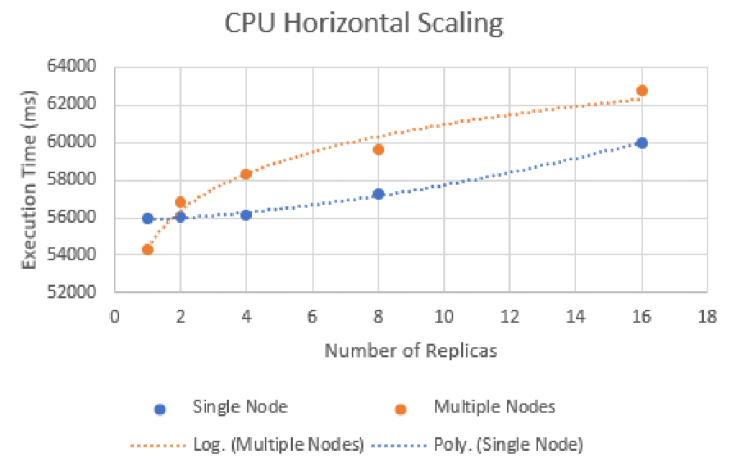
\includegraphics[width=0.65\columnwidth]{Images/Related_work/Hyscale_1.PNG}
%\end{center}
%\caption{Horizontal scaling response times for CPU tests~\citep{hyscale}}
%\label{fig:hyscale1}
%\end{figure}
%
Wong compares HyScale to the standard autoscalers in Kubernetes. A first disadvantage of Kubernetes noted by Wong is that its default scaling solutions only consider one resource when making scaling decisions. Second, Wong explains how the Kubernetes autoscalers often lead to sub-optimal configurations. 
HyScale differs from the default Kubernetes HPA in two ways: the use of vertical scaling and the consideration of multiple metrics to make scale decisions. 
Wong's experimental results show that HyScale outperforms Kubernetes for bursty workloads. For non-bursty workloads, their performance is similar
~\citep{hyscale}.

When comparing horizontal and vertical scaling for CPU intensive workloads, Wong describes that Docker's \textit{cpu-shares} mechanism can be used to ``induce a form of vertical scaling, as increasing or decreasing shares directly correlate with an increase or decrease in CPU resource allocation to a container''~\citep{hyscale}. When comparing their solution to Kubernetes, however, they only consider the Kubernetes HPA, without mentioning these \textit{cpu-shares}. This paper evaluates the effects of combining the HPA with the \textit{cpu-shares} mechanism in Kubernetes. 
